% Created 2013-11-06 Wed 10:27
\documentclass[11pt]{article}
\usepackage[utf8]{inputenc}
\usepackage[T1]{fontenc}
\usepackage{fixltx2e}
\usepackage{graphicx}
\usepackage{longtable}
\usepackage{float}
\usepackage{wrapfig}
\usepackage{soul}
\usepackage{textcomp}
\usepackage{marvosym}
\usepackage{wasysym}
\usepackage{latexsym}
\usepackage{amssymb}
\usepackage{hyperref}
\tolerance=1000
\providecommand{\alert}[1]{\textbf{#1}}
\usepackage{varioref}

\usepackage{setspace}
\onehalfspacing

\title{03-60-311 Final Report}
\author{Matt Clifford, Jeff Drake, Jeremy High, Stephen Nusko, Matt Renaud}
\date{\today}

\begin{document}

\maketitle

\vspace{1.5in}

\begin{center}
  University of Windsor

  Computer Science Department
\end{center}

\newpage
\setcounter{tocdepth}{3}
\tableofcontents
\vspace*{1cm}

\section{Introduction}
\label{sec-introduction}

\subsection{Problem Statement}
\label{sec-prodlem-statement}

\subsection{Project Overview}
\label{sec-project-overview}

\subsection{Release Notes Summarizing the Last Transition}
\label{sec-release-notes}

\section{Software Requirements}
\label{sec-software-reqs}

\section{Design Specification}
\label{sec-design-specs}

\subsection{Software Architecture (Chapter 6)}
\label{sec-software-architecture}

	As suggested in Chapter 6 Section 6.2 of the textbook, a full 4 + 1 view of the architecture is overly extensive for an agile approach.
	We therefore will focus on some patterns that we found helpful in understanding the design of our system.
	\subsubsection{Model-View-Controller (Section 6.2)}
		The Model-View-Controller pattern was found to be very applicable, and useful in separation of the data and representation. 
		See figure 6.4 below. 
		The model part is based on our SQLite database, while our controller was the Django framework which handled all HTTP requests and application logic. 
		While the use of Ajax allowed for dynamically generating the page and forms as needed. \\
		\centerline{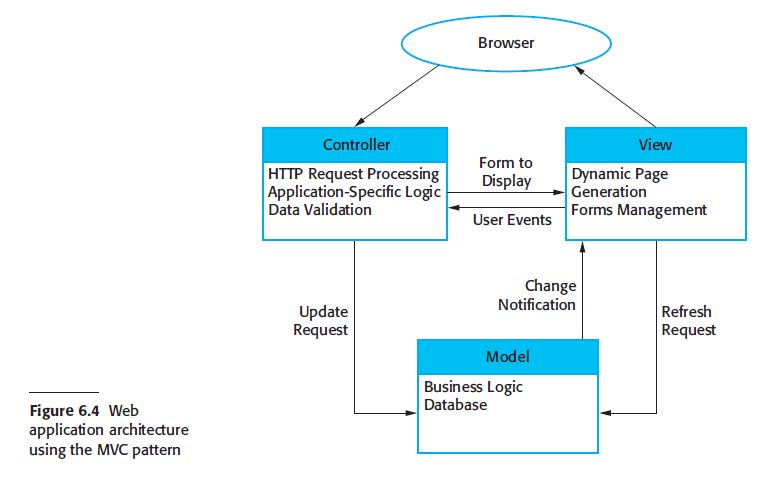
\includegraphics[scale=0.5]{./images/MVC}}
	\subsubsection{Application architectures}
		When we discussed the design of our application and studied system outlines, we found from Section 6.4.2 that our program as a web application is very much an information system, with a shared database which connects through layers to the user. 
		See figure 6.17 below. 
		The first two layers of the figure are equally valid for our system, and the remaining two need only minor name changes. 
		Our database connects to the Django framework which helpfully manages both of the middle layers.
		While doing this Django also allows user applications to be seperated from data management, and thus keeps the layers seperate. \\
		\centerline{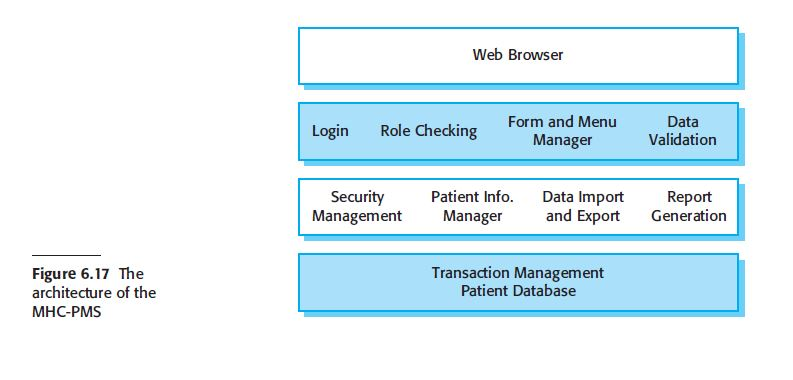
\includegraphics[scale=0.5]{./images/TPIS}}

\subsection{Sequence Diagrams }
\label{sec-sequence-diagrams}
Proceeding every sequence diagram there will be a fully dressed use case outlining the situation for the sequence diagram. 
	These go together as they are both in Chapter 5 in Section 5.2 "Interaction models" of the textbook.
	\subsubsection{Login and Registering}
		\begin{longtable}{| l | p{8cm} |}
			\hline
			Use Case Name & Logging in or Registering \\ \hline
			Scope & Buchladen Book system \\ \hline
			Primary Actor & User \\ \hline
			Stakeholders and Interests & \begin{itemize}
							\item The user wishes to easily login and a new user wants to be able to get set up quickly.
							\item The user wants their information secure.
						     \end{itemize} \\ \hline
			Preconditions & None \\ \hline
			Success Guarantee & The login button will change to their username if successful. \\ \hline
			Main success Scenario & \begin{enumerate}
							\item The user clicks the login button.
							\item The user proceeds to fill out the information.
							\item The user clicks submit.
							\item The system then checks to see if the user gave valid information or if the username is currently free, and in that case registering and saving it to the database, before proceeding with logging them in.
							\item A logged in homepage is then shown to the user.
						\end{enumerate} \\ \hline
			Extensions & 2a) The user could input the wrong information, in this case they should be prompted to restart at step 2. \newline 4a) The system could have trouble reaching the database, in this case the user should be informed to try back in a little bit. \\ \hline
			Special Requirements & None \\ \hline
			Technology and Data Variations List & None \\ \hline
			Frequency of Occurrence & Zero to multiple times per day, based on popularity of system. \\ \hline
			Miscellaneous & None \\ \hline
		\end{longtable}
		\centerline{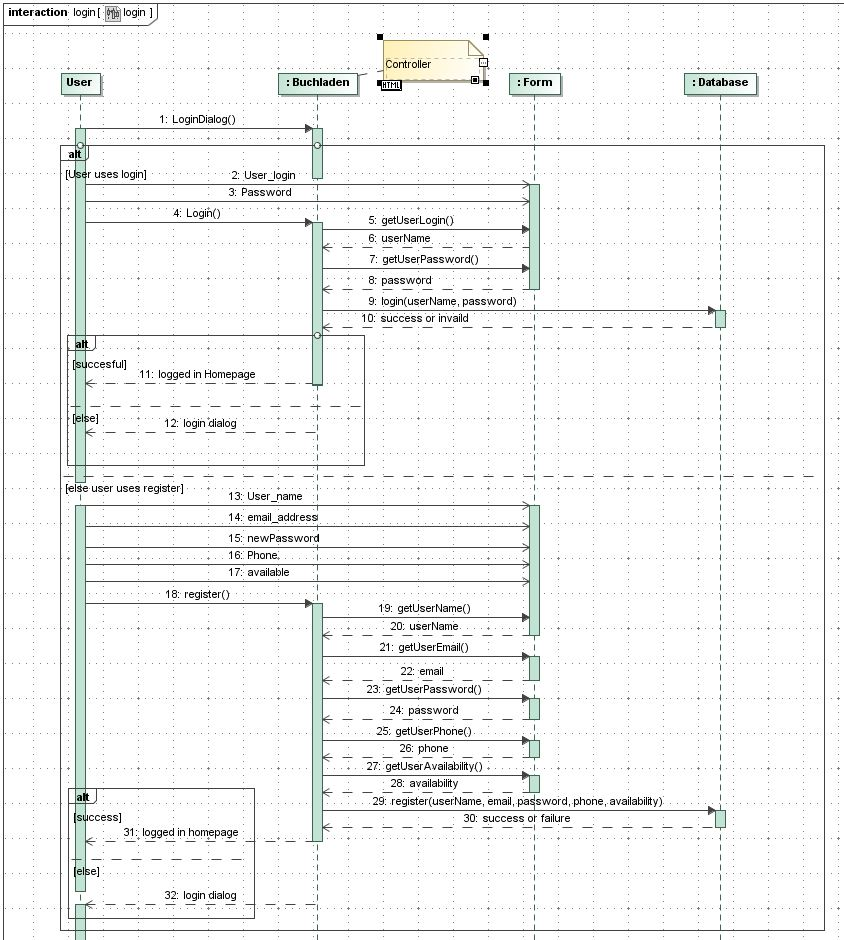
\includegraphics[scale=0.75]{./images/loginAndRegister}}
	\subsubsection{Posting a Book}	
		\begin{longtable}{| l | p{8cm} |}
			\hline
			Use Case Name & Posting a book \\ \hline
			Scope & Buchladen Book system \\ \hline
			Primary Actor & User \\ \hline
			Stakeholders and Interests & \begin{itemize}
							\item The user wishes to easily post a book for sale.
							\item The admins wish to have only relevant postings.
							\item Other users wish to see the information as quickly as possible and be able to purchase the book.
						     \end{itemize} \\ \hline
			Preconditions & The user must be registered in the system, and logged in. \\ \hline
			Success Guarantee & The user will be informed that the posting was successful, and the book will be visible to the public. \\ \hline
			Main success Scenario & \begin{enumerate}
							\item The user clicks the post button.
							\item The user proceeds to fill out the information.
							\item The user clicks submit.
							\item The system then retrieves the inputted data.
							\item The system saves the new book into the database.
							\item A confirmation webpage is shown to the user.
						\end{enumerate} \\ \hline
			Extensions & 1a) The user could not be logged in, in this case the post dialog will fail to open, and the user will have to log in before proceeding with step 1 \newline
			2a) The user could input the incorrect information. The user will be able to verify and edit the information at a different page. \newline
			4a) The system could have trouble reaching the databse, in this case a message should be displayed informing the customer to try again later. \\ \hline
			Special Requirements & None \\ \hline
			Technology and Data Variations List & None \\ \hline
			Frequency of Occurrence & Zero to multiple times per day, based on popularity of system. \\ \hline
			Miscellaneous & None \\ \hline
		\end{longtable}
		\centerline{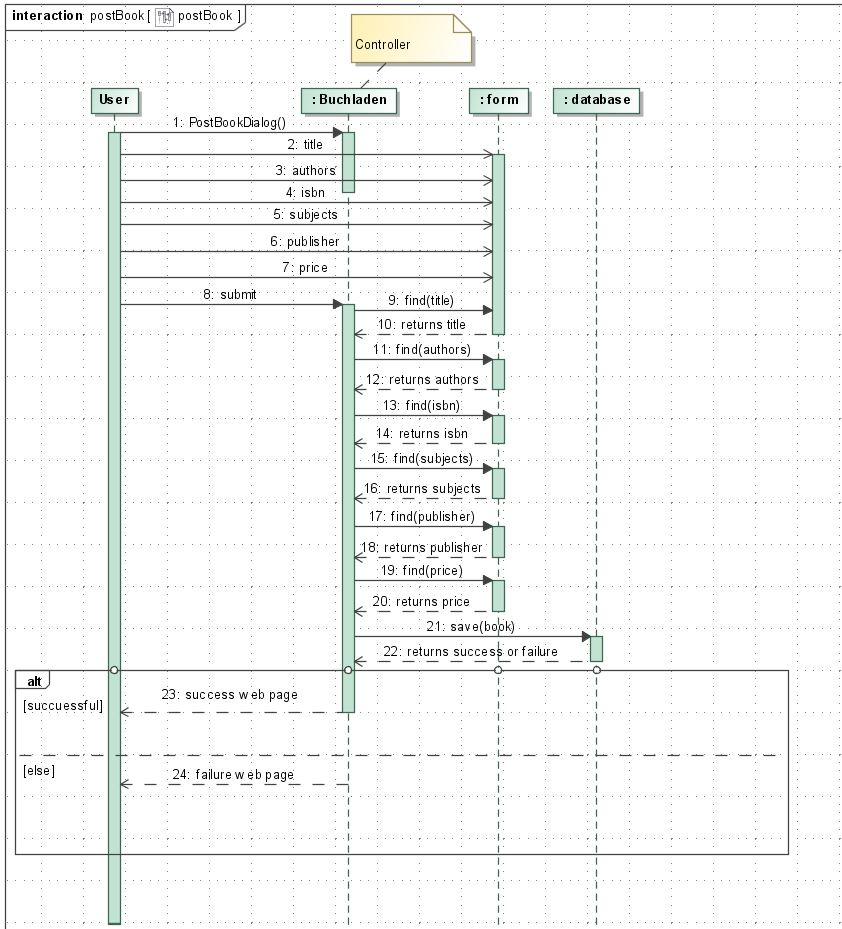
\includegraphics[scale=0.75]{./images/postBookSequenceDiagram}}
	\subsubsection{Contacting a Seller}
		\begin{longtable}{| l | p{8cm} |}
			\hline
			Use Case Name & Contacting a seller \\ \hline
			Scope & Buchladen Book system \\ \hline
			Primary Actor & User \\ \hline
			Stakeholders and Interests & \begin{itemize}
							\item The user wishes to contact a seller of a book for sale.
							\item The admins wish to facilitate the sale without giving away more than required information about the poster or user.
							\item The seller wishes to be able to sell his book quickly and easily.
						     \end{itemize} \\ \hline
			Preconditions & The seller must have posted a book. \\ \hline
			Success Guarantee & When the user sends teh email they will receive a confirmation page. \\ \hline
			Main success Scenario & \begin{enumerate}
							\item The user searches for the book they want and clicks contact seller.
							\item The user fills in their information for contacting, and then writes the email.
							\item The user clicks submit.
							\item The system then retrieves their message and emails it to the seller.
							\item The user is then directed to a confirmation page.
						\end{enumerate} \\ \hline
			Extensions & 2a) The user could choose to contact the seller by phone, this is allowed and the user should proceed by dialing the sellers number. \newline 
			4a) The system could have trouble reaching the database, in this case the user should be informed to try back in a little bit. \\ \hline
			Special Requirements & None \\ \hline
			Technology and Data Variations List & None \\ \hline
			Frequency of Occurrence & Zero to multiple times per day, based on popularity of system. \\ \hline
			Miscellaneous & None \\ \hline
		\end{longtable}
		\centerline{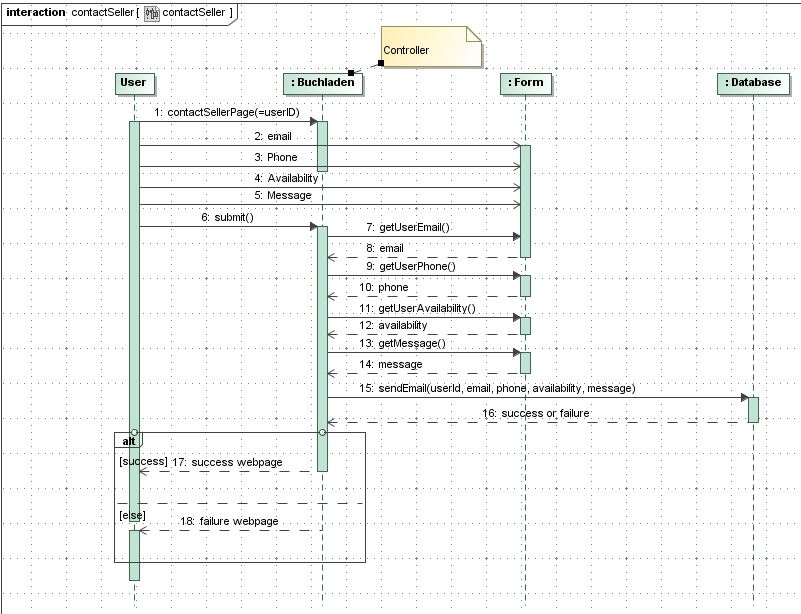
\includegraphics[scale=0.75]{./images/contactSellerSequence}}
	
\subsection{Class Diagrams (and their relationships)}
\label{sec-class-diagrams}

\section{Technical Documentation}
\label{sec-technical-docs}

In this section we present several technical aspects of the online
used book store that we have designed and developed.  We begin by
discussing the platform that we used to deploy the web application,
any setup required for the environment, as well as the application
framework and the major programming languages that have been used in
the implementation. We then go on to discuss some of the tools and
algorithms that we used throughout the development cycle and conclude
the section with an overview of the database tables and schema that we
used for the persistent storage of data.

\subsection{Programming Language and Platform}
\label{sec-language-and-platform}

We made the decision to deploy our web application on the GNU/Linux
platform, it is currently hosted on the University of Windsor's
Student Operated Computing Resources (SOCR) server which is running
Debian Linux. The reason why Linux was chosen as the development
platform is because most servers run some distribution of Linux which
made the decision quite simple.

After we had decided on the platform, we were faced with the challenge
of selecting a programming language and a framework to use to build
the application. Since we were writing software for the web, we
obviously needed to use HTML and CSS, but we still needed to decide on
the language to use for the backend. All of the members of the group
had previous experience developing web applications using PHP, and all
unanimously agreed that although PHP has become a defacto standard for
web development, using a more structured language and a framework
would ease the development and debugging process and as a result we
decided to use Django, a web application framework written in Python.

\subsubsection{Django}
\label{sec-django}

Although none of our group members were incredibly familiar with
Python, we anticipated that the time saved by using a framework would
outweigh the time required to learn a new language and become familiar
with the architecture of the system. In the end, making the choice to
use Django was an excellent decision and allowed us to focus more of
our time on implementing features than on writing all aspects of the
system from the ground up and reinventing the wheel.

Django is described on its website (see Section~\vref{sec-reference})
as:

\begin{quotation}
  ... a high-level Python Web framework that encourages rapid
  development and clean, pragmatic design.
\end{quotation}

and follows the Model, View, Controller software pattern. This pattern
allows for the separation of concerns and allows for the writing of
more modulal, maintainable code. The backend that interacts with the
database is separated from the code that is used to generate the front
end view that the end user sees. This allowed us throughout the
development process to have different people working on different
areas and features of the application at the same time and once a
component was finished it could be seamlessly included into the
system.


\subsection{Ajax}
\label{sec-ajax}

In addition to the languages that we used, we also took advantage of
several web technologies in order to modernize our website. The one
that we used the most was Ajax (Asynchronous JavaScript and Xml),
which allows for requests to be made to the server and updates to be
made to the page without the page having to be reloaded. This allowed
us to update the search results as search terms were being entered and
the page could be dynamically updated based on the results.

Many web sites such as Facebook and Google use Ajax to make sure that
the content of the page is up to date without requiring any page
reloads. Having this as part of a website is something that is almost
mandatory to have the feel of a modern web site.

In addition to having a smoother user experience, using Ajax improves
the performance of the site as well as decreasing bandwidth usage. By
sending sending only the results to the client and not all of the HTML
and CSS over again saves bandwidth as well as decreases the time
required to view the latest results. 

\subsection{Development Tools}
\label{sec-development-tools}

In order to develop the web application, some of the members of our
group used a python development environment called PyCharm which has
built in Django support to ease the development of the python
code, while other members of the group used text editors to write the
HTML and CSS required to give the site its structure and style.


\subsection{Database Tables and Schema}
\label{sec-database-schema}

\section{User Documentation}
\label{sec-user-docs}

\section{Software Test Plan}
\label{sec-software-test-plan}
	\subsection{Overview of Testing}
		When designing the software test plan it is important to remember the environment that it will be made, and released in.
		We will start with an exploration of the purpose, expectations, and environment, before proceeding with an in-depth analysis of all the software testing processes used. \\
		\centerline{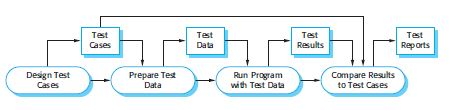
\includegraphics[scale=0.75]{./images/testProcesses}} 
		Figure 8.3 from the textbook, showcases a model for software testing.
		All section numbers in the proceeding discussion refer to Chapter 8 in Software Engineering by Ian Sommerville, Ninth Edition.
		From the introduction to Chapter 8, we will briefly cover that the software is good for the intended use, by looking at the following.
		\subsubsection{Software Purpose (Intro)}
			The purpose of the software is to provide students of the local campus a common place to post and share unneeded textbooks.
			As well as provide a method for users to contact and arrange the purchase of textbooks they need for their courses. 
			The system does not control a safety-critical system; rather it brings people together for ease of use. 
			The software must be reliable in having the correct information for contacting users, and the current offerings of books.
		\subsubsection{User Expectations (Intro)}
			Users expect a seamless experience of browsing for books, contacting sellers if the price point seems reasonable.
			However because it's a low key system, no personal information besides the user's name and email address and possibility phone numbers are stored.
			Users will understand if the website or server fails and must be restarted during the launch.
			However as the system becomes more popular it will be important to upgrade servers and clamp down on bugs because system failures will not be tolerated over other competitors.

		\subsubsection{Marketing environment (Intro)}
			There are quite a few competing products including companies such as, Kijiji, Amazon, saveontextbooks, etc.
			However there is no website that focuses just on our personal campus so our product fills a niche that exists.
			So this product will be the true first in its own little area, but with other broader competitors.
			It therefore requires a decent level of reliability, but some down time or errors will be acceptable as long as they are not to major.

	\subsection{Development Testing (Section 8.1)}
		As described in 8.1 Development testing includes any testing down during development by the team working on the system. 
		For this reason I've included software inspections from the introduction, as well as standard testing approaches from section 8.1.
		Our testing approach during development was based on each member was responsible for using a defect testing process to find their own errors, but as well we had some helpful tools and tests in place to help ensure defects were found. 
		We also used pair programming to have concurrent inspections ongoing.

		\subsubsection{Software Inspections (Intro)}
			\centerline{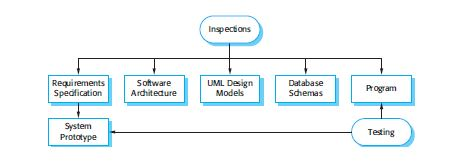
\includegraphics[scale=0.75]{./images/inspections}} 
			The above image is figure 8.2 from the textbook. Jeffery Drake was in charge of inspecting and analyzing the software architecture, and database schemas. 
			Jeffery found sections of code that didn't meet our expected standard for maintainability and efficiency. 
			This caused many refactors in keeping with certain agile methods to improve the reuse of code from Django, while improving the overall architecture.  
			Matt Renaud was constantly reviewing and analyzing the requirements specification based on the current project, and on iteration meetings with our client as well as the various system prototypes. 
			Changing the specification and the working design models as needed. 
			Every member was responsible for at inspections of their own portions of code, and ensuring the entire system still worked together correctly.
		\subsubsection{Unit Testing (Section 8.1.1)}

			Each individual Model we created was tested using Django's automated testing suite, in the style of JUnit tests. 
			Each class and function within was tested. 
			Test cases were developed based on the real data that was taken and stored in a test database to ensure no tests could affect production data. 
			Expected output was worked out by hand, and then tested against the program output. 
			Test reports are then automatically generated by Django. 

		\subsubsection{Component Testing (Section 8.1.3)}

			Some of the components such as Users model, and Forms have innate testing suite, but other models like our book which includes various sub models including Author, and Subjects were tested for their integration and correct overall function. 
			Again Test cases were developed to ensure that each situation within the model was tested, multiple authors, multiple subjects, or just single, as well as verification that there can be no book without at least one of the previous parts filled out.

		\subsubsection{System Testing (Section 8.1.4)}

			System testing is done almost exclusively through Django's framework; there are 999 tests that test the entire subset of the program interface. 
			Every template, user, default webpage also including our unit and component tests is also included in that number. 
			This allows us to have a relatively quick method to ensure our current system build is up to specifications.

	\subsection{Release Testing (Section 8.3)}

		Unfortunately as described in section 8.3 of the textbook we have no separate team to look over our program for formal release testing.
		However when talking with our client it was stated that the product should be to the level of or close to finished prototype so full release testing would be done at a later date. 
		However parts can be implemented currently. 

		\subsubsection{Requirements-based Testing (Section 8.3.1)}

			All of our Unit and component testing contain requirement based testing. 
			Ensuring the correct output that is expected is received. 
			However other requirements such as performance and scenario require a different approach then unit and component testing can provide.

		\subsubsection{Scenario Testing (Section 8.3.2)}

			Must feature was tested with a use case, and some important features had a sequence diagram designed. 
			They have been attached earlier in this report. 
			Testing was done to ensure the main success story of the use case flowed correctly and achieved the desired aim.

		\subsubsection{Performance Testing (Section 8.3.3)}

			Again because full release testing is not possible, we have only implemented and tested some parts of the performance of the system. 
			These can be split into the following.

		\subsubsection{Failure Behaviour (Section 8.3.3)}

			When the service is not running on the server the response from the server renders a page explaining the page is temporarily unavailable and will be back later. 
			This will inform the customer of the issues and let the system admin have some time to find errors and correct them.

		\subsubsection{Stress Testing (Section 8.3.3)}

			We have been running our website throughout the various development versions uploaded and running in a production environment at Buchladen.uwinsocr.ca with no crashes so far. 
			Response time is quick and usability and reliability has been found to be excellent. 

	\subsection{User Testing (Section 8.4)}
		We will split up user testing into two sections one based on the basic alpha and beta testing and then an entire section to acceptance testing, these come from section 8.4 of the text book.
		\subsubsection{Alpha Testing}

			Every member of the development team was responsible for defect testing, and validation testing of the current tasks they were implementing in that particular iteration. 
			Other members would also inspect the other features that were implemented to ensure no defects were missed, and to validate the correct usage, or attempt to find defects.

		\subsubsection{Beta Testing}

			Friends and the client were shown the system and encouraged to comment on anything they saw. 
			The team asked them to try and think of exceptions and invalid inputs they could use. 
			They were asked to comment on the functionality and the aesthetics, and changes were made to the project direction resulting from their recommendations.

	\subsection{Acceptance Testing (Section 8.4)}

		\subsubsection{Acceptance Criteria}

			The client agreed to requirement-based acceptance testing. 
			Many features must be in working order including; registration, login, posting books, contacting sellers, and administration abilities.

		\subsubsection{Acceptance Testing Plan}

			We will provide a suite of unit and component tests, as well system integration tools, to ensure desired functionality. 
			There will also be use case and inspections of the system's design and performance.

		\subsubsection{Acceptance Tests}
			\begin{enumerate}
				\item Unit tests
				\item Component tests
				\item System integration
				\item Inspections
				\item Scenario cases
			\end{enumerate}

		\subsubsection{Run Acceptance Tests}
			All tests have been run and passed. No major issues were found.

		\subsubsection{Reject/Accept System}
			The system has been submitted to the client for final review and acceptance.
\section{Reference}
\label{sec-reference}

\begin{description}
\item[Python Tutorial] \href{http://docs.python.org/3/tutorial/}{http://docs.python.org/3/tutorial/}
\item[Django Homepage] \href{https://www.djangoproject.com/}{https://www.djangoproject.com/}
\item[Unit Test] \href{https://docs.djangoproject.com/en/dev/topics/testing/}{https://docs.djangoproject.com/en/dev/topics/testing/}
\item[Source] \href{https://github.com/iaefai/Buchladen}{https://github.com/iaefai/Buchladen}
\item[RedMine]
  \href{https://redmine.cs.uwindsor.ca/projects/team10/}{https://redmine.cs.uwindsor.ca/projects/team10/}
\item[Django Nap] \href{https://github.com/funkybob/django-nap}{https://github.com/funkybob/django-nap}
\item[Json] \href{http://www.json.org/}{http://www.json.org/}
\item[JQuery-Ajax] \href{http://api.jquery.com/jQuery.ajax/}{http://api.jquery.com/jQuery.ajax/}
\end{description}


\end{document}
